\chapter{The Standard Model of Particle Physics}
\label{chap:intro}

The first recorded use of the word ``elements'' is by Empedocles in the 5th Century B.C. He proposed that 4 substances; earth air, fire, water, make up all of nature and can explain all the complexity of matter. 
This constitutes one of the first attempts at reductionist thinking in order to explain the world. Reductionist thinking has been very influential in modern physics, especially in the area of particle physics. 
The ability to break down what we previously thought were `` elementary'' particles into the constituent parts has led to many great discoveries. 
The electron, the first truly elementary particle to be discovered, was first hinted at in the 1869 discovery of cathode rays by Johann Wilhelm Hittorf. 
In 1897 , JJ. Thompson showed that cathode rays are streams of a previously unidentified negatively charged particle, which would later be named the electron. 
In 1911, Charles Wilson developed a cloud chamber which allowed for the first photographic evidence of electrons. Protons would be discovered in 1917 and then the neutron would be discovered in 1935. 
This launched a century of discovery that would culminate in 2012 with the discovery of the Higgs Boson, which was one of the last pieces of the puzzle in order to explain 3 of the 4 fundamental forces in nature. We call it the Standard Model of Particle Physics.

The Standard Model(SM) of Particle Physics is the theory that explains all the known particles and the forces that govern their behavior, with the VERY notable exception of gravity. 
This is quite an astonishing statement because there are hundreds of known particles and to be able to explain them in a relatively succinct manner is quite the accomplishment of modern science. 
One way to represent this is a useful diagram that has become popular in explaining the SM, see Figure \ref{fig:fig_SM}. 
% Figure 1-1
\begin{figure} %  figure placement: here, top, bottom, or page
    \centering
 %   
\includegraphics[width=\textwidth,height=\textheight,keepaspectratio]{fig_2-1}
    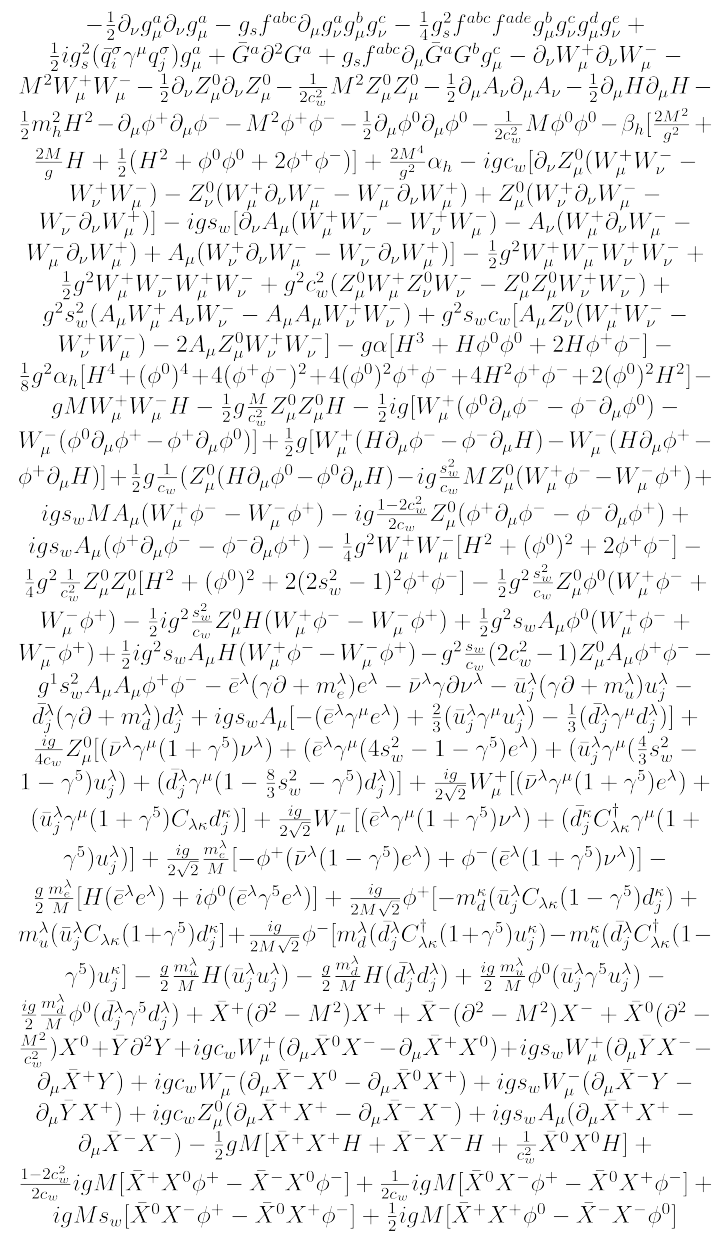
\includegraphics[scale=0.5]{SMlagrangian.png}
    \caption{The lagrangian form of the the Standard Model}
    \label{fig:fig_1-1}
 \end{figure}

 % Figure 1-1
\begin{figure} %  figure placement: here, top, bottom, or page
    \centering
 %   
\includegraphics[width=\textwidth,height=\textheight,keepaspectratio]{fig_2-1}
    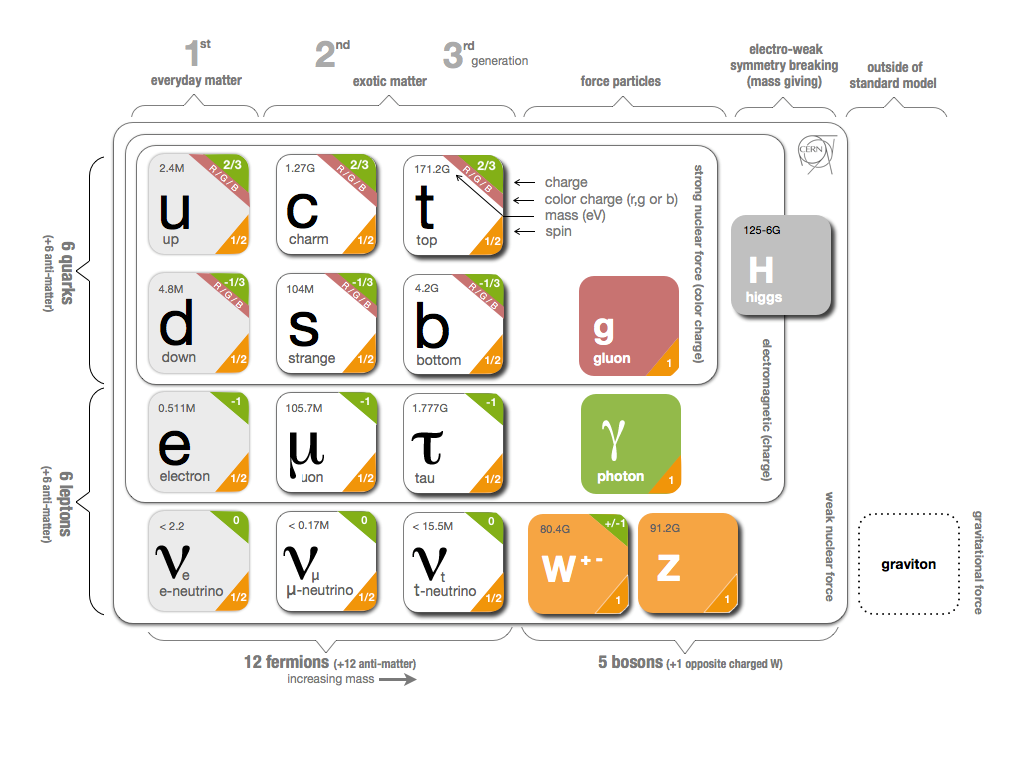
\includegraphics[scale=0.4]{SMinfographic_image.png}
    \caption{A graphical depiction of the Standard Model}
    \label{fig:fig_SM}
 \end{figure}
\section{Standard Model Particles}
\subsection{Leptons}
Starting with the electron, we can begin to fill out the SM with two other particles that are in some sense just heavier version, the muon ($\mu$) and the tau ($\tau$). 
They all have charge of $-1$ \footnote{The unit of 1 here represents $-1.602$ x $ 10^{-19} Coloumbs$ }. One can see that the muon and the tau have masses roughly 200 and 4000 times that of the electron.
There also exists a pair neutrino, denoted as $\nu$, for each of these leptons which will complete our lepton table in the SM. The electron, muon, and tau neutrinos all have 0 charge and are supposed to be massless in the SM.
You will see that on the table in Figure \ref{fig:fig_SM} each of the flavors of neutrino have a mass bound of less than some value. This is because various experiments have shown that the neutrinos have some mass.
Since the mass of the neutrino is not predicted by the SM, we expect that some beyond Standard Model (BSM) explanation exists. Each of these particles has an anti-particle which is notated with a bar over the symbol. These are the $\bar{e}, \bar{\mu}, \bar{\tau}, \bar{\nu_{e}}, \bar{\nu_{\mu}}, \bar{\nu_{\tau}}.$

All the leptons also have other properties which are important to mention. The first is something called ``spin''.
This represents the intrinsic angular momentum of the particle. It is a purely quantum property so one should not think of it as a measurement of how fast the particle rotates. 
Rather it is one component of the total angular momentum of the particle. However, the classical analogy is useful. Just as something can spin in multiple directions classically, this quantum notion of spin has two directions we denote as positive and negative.
This spin can come in quantities which have whole units, 0,1,2, and in half units of, $\frac{1}{2}$. The leptons mentioned above all have spin of positive or negative $\frac{1}{2}$.
Particles with integer half spin, like leptons, are called fermions.

There is another important property which we call helicity (also called handedness), defined as the sign of the particles spin vector projected onto its momentum vector.
Usually, negative helicity is referred to as left-handed and positive helicity is referred to as right-handed. This property plays an important part in the calculations of the SM and therefore is not a trivial quantity.
Particles with different handedness can behave differently. For example, while the massive leptons can all be either left or right handed, the neutrinos are all left handed and the anti-neutrinos are all right handed.
This phenomenon currently has no explanation in the SM.

\subsection{Hadrons}
There are many more particles that have been discovered in the past 100 years. These have been meticulously detailed in a reference made by the Particle Data Group (PDG) and can be bought in a large textbook form or a small quick reference. 
However, the majority of these particles are composite particles, called Hadrons, that are made up of one of the six quarks seen in Figure \ref{fig:fig_SM}.
These quarks also come in three groupings or ``generations''. \footnote{Why only 3? The SM theory requires 3 generations to preserve CP violation. However, this is a minimum and there is nothing preventing a 4th or 5th generation except we have not found them.}
The quarks are the up (u) and down (d), stange (s) and charm (c), and bottom (b) and top (t). The u, c, and t quarks all have charge of $+ \frac{2}{3}$ and the d, s, and b quarks all have charge of $-\frac{1}{3}$.
They have their own masses, spins, and anti-particles (also denoted with a bar over the usual symbol), like the leptons do. They all have spin $\pm \frac{1}{2}$ so they are also fermions.\\

The quarks have an extra property that is unique, called color. This is another quantum property but unlike quantum spin, there is not a very good classical analogy.
It can be thought of as a kind of ``charge'', but it has three different types, red, green, and blue. There also exists anti-red, anti-green, and anti-blue for the anti-quarks.
The color of a quark is not directly detectable and must be determined through the quarks interactions. 
It is also not possible for quarks to exists in anything but color neutral combinations. This will be further explained in the section on forces.
These color neutral combinations make up a lot of the particles in nature. For example, the proton is made of two u and one d quark. Therefore, it has a charge of $\frac{2}{3} + \frac{2}{3} - \frac{1}{3} = +1$ because of this fact.
The neutron on the other hand, is made of two d and one u quark. This combinations creates a neutral electric charge. 
Since the quarks always come in color neutral combinations, the fractional charges of the quarks also cannot be directly detected because all of the color neutral combinations also have whole numbers of electric charge.

\subsection{Bosons}
There are 5 bosons listed in figure \ref{fig:fig_SM}. They are the photon, the gluon, the $W^{\pm}$, the Z and the Higgs bosons.
Unlike the fermions, which all have spin $\pm \frac{1}{2}$, the bosons all have a unit spin of 1\footnote{There exists the theoretical possibility of spin 0 or 2 bosons but none has been detected so far}.
The photon and the gluon are massless, while the W, Z, and Higgs bosons have mass. This is not an accident and will be further explained in the following section on forces. So why do we distinguish fermions from bosons?
The reason is that they fundamentally behave differently. The fermions are what everyday matter is made of but the bosons are what mediate the interactions between fermions. 
To put it simply, the bosons act on the fermions in what we call the forces of the SM.\\

\section{Standard Model Forces}
There are three fundamental forces that the SM explains, electromagnetism, the weak force, and the strong force, with the obvious absence of gravity.
While gravity was one of the earliest forces to be quantified, it has resisted our attempts at understanding it at a quantum level.
To date, our inability to reconcile the current theory of gravity with the quantum nature of the SM is one of the most vexing problems facing physics.

The forces of the SM interacting with particles are mediated by ``force carrying'' particles.
We can consider a very basic situation where two particles are launched at each other. Let us consider like charges so that the two particles will repel each other.
Then we can construct an infinite sum of all the possible interactions between the two particles that start in an initial state, $i$, and end in some final state $f$ as:
\begin{equation}
S_{i \rightarrow f} = \sum_{n=0}^{\inf} I^{n} 
\end{equation}
where each term $I^{n}$ is a different possible interaction between the two particles. The first term is not interesting because it is the term that denotes the two particles not interacting.
So the first interacting term is then:
\begin{equation}
I^2 =  (\pm)^n \bar{\psi(x)} V \psi(x)\bar{\psi(x')} V \psi(x') \int (\frac{dk}{2 \pi})^4 \frac{-g_{\mu \nu}}{k^2 - i0} e^{-ik(x-x')}
\label{eq:eq_baseIntegral}
\end{equation}
where the terms $\psi, \bar{\psi}$ refer to the two particles initial and final states and the V term is the interaction vertex. 
The $\frac{g_{\mu \nu}}{(k^2 - i0)}$ term in the integral is a propagator which denotes the force interaction between the two particles (in this case the electromagnetic force is mediated with a photon). The integral is computed over all incoming and outgoing momenta, $k$.
\\

\begin{figure} %  figure placement: here, top, bottom, or page
   \centering
      \feynmandiagram[horizontal=a to b] {
      i1  [particle=$\phi$] -- [fermion] a -- [fermion] i2  [particle=$\phi$],
      a -- [photon, edge label=\(\gamma\),] b,
      f1 [particle=$\bar{\phi}$] -- [fermion] b -- [fermion] f2 [particle=$\bar{\phi}$],
      };
   \caption{An example Feynman Diagram}
   \label{fig:fig_1-3}
\end{figure}


This equation, while precise and useful for direct computation, is not very instructive and can be put in a pictorial representation that is much easier to read.
These representations are called Feynman Diagrams. Each term in the infinite sum above can be drawn with a Feynman diagram allowing us to see all the necessary components for the interaction.
More importantly, this representation does not lose any of the preciseness of the equations, they are essentially one and the same. 
\begin{equation}
   \feynmandiagram[inline=(d.base),horizontal=d to b] 
   {a -- [fermion] b -- [fermion] c,b -- [boson] d [particle=\(\gamma\)],
   };
   = V
   \label{eq:eq_Vertex}
\end{equation}
Equation \ref{eq:eq_Vertex} is the mathematical expression for a vertex. A vertex is essentially the interaction point between two particles.
One can build the diagram in Figure \ref{fig:fig_1-3} by combining two vertices and correctly writing the corresponding propagator.

The simplest Feynman diagram (which is the first term in the sum) allows us to build an intuition of what is dominantly happening, which is that two particles are coming together, combining into an intermediate particles, and then that intermediate particle is decaying into two particles.
This general description is actually very powerful. One can construct any number of particle combinations in such a way as they annihilate (or merge) into an intermediary particle and then decay into two (maybe even more) new particles. 
This ability to write down particle interactions based on a set of rules, which we will describe in following sections, is the foundation of the SM. We can classify three of the four fundamental forces of nature by constructing rules around the combination of vertex diagrams with particular intermediate particles.
These intermediate particles are usually the bosons that govern a force that the particles are interacting with each other through. 


\subsection{Electromagnetic Force}
Classically, Maxwell's equations do a very good job describing classical electromagnetic experiments. However, to describe phenomena involving elementary particles that are moving with relativistic energies, we need a quantum theory. 
The quantum theory of electromagnetism is called \textit{quantum electrodynamics}. This theory governs all of the possible interactions between the photon, the propagating particle of the electromagnetic force, and any particle that interacts with the photon.
Recall that the interaction vertex is the base of the rules for constructing Feynman diagrams and the interaction vertex for the photon is given in equation \ref{eq:eq_EMVertex} as:
\begin{equation}
   \feynmandiagram[inline=(d.base),horizontal=d to b] 
   {a -- [fermion] b -- [fermion] c,b -- [boson] d [particle=\(\gamma\)],
   };
   = i e \gamma^{\mu}
   \label{eq:eq_EMVertex}
\end{equation}
The equation for the propagating photon is:
\begin{equation}
   \gamma =  \frac{g_{\mu \nu}}{(k^2 - i0)}
\end{equation} 
which when combined together and integrated over all momenta, can be made into an equation which is similar in form to \ref{eq:eq_baseIntegral}.

A quick example of how powerful these tools can be is electron-positron annihilation. If a positron and an electron interact through a photon we will get the diagram shown in Figure \ref{fig:fig_1-4}.
We can also use some rules from classical electromagnetism, i.e charge is conserved, to tell us if this process is possible in nature. In this example, the total charge of the incoming particles is $1 + (-1) = 0$. 
The photon has charge $= 0$ so then this will conserve charge and is possible in nature. Using charge conservation as another rule we can construct other diagrams by just switching out the electron-positron pair with another lepton, anti-lepton pair.
One classic example is to use the muon and anti-muon which yields the diagram seen in Figure \ref{fig:fig_1-5}. QED is very well tested in modern day experiments and there are no known expected differences between it and the SM.


\begin{figure} %  figure placement: here, top, bottom, or page
   \centering
      \feynmandiagram[horizontal=a to b] {
      i1  [particle=$e^{-}$] -- [fermion] a -- [fermion] i2  [particle=$e^{+}$],
      a -- [photon, edge label=\(\gamma\),] b,
      f1 [particle=$e^{+}$] -- [fermion] b -- [fermion] f2 [particle=$e^{-}$],
      };
   \caption{Electron positron annihilation.}
   \label{fig:fig_1-4}
\end{figure}

\begin{figure} %  figure placement: here, top, bottom, or page
   \centering
      \feynmandiagram[horizontal=a to b] {
      i1  [particle=$e^{-}$] -- [fermion] a -- [fermion] i2  [particle=$e^{+}$],
      a -- [photon, edge label=\(\gamma\),] b,
      f1 [particle=$\mu^{+}$] -- [fermion] b -- [fermion] f2 [particle=$\mu^{-}$],
      };
   \caption{Electron positron annihilation into a muon and anti-muon pair.}
   \label{fig:fig_1-5}
\end{figure}

\subsection{Strong Force}

The Strong Nuclear Force, or strong force for short, governs the interactions inside of hadrons like the proton and neutron. The mediator, or propagator, for the strong nuclear force is the gluon. The theory governing this force is called \textit{Quantum Chromodynamics}.
It can be said that QED is the theory of electrically charged interaction and the analogy for QCD is that it is the theory for colored interactions \footnote{Recall that I described quarks as also having a color charge.}.
Unlike the photon, which since it has no charge it cannot couple to itself, the gluon has a color charge and so the interaction vertices possible to make Feynman diagrams are slightly more complicated and are shown in Figure \ref{fig:fig_1-6}.
\begin{figure} %  figure placement: here, top, bottom, or page
   \centering
   \begin{subfigure}[t]{0.49\textwidth}
      \feynmandiagram[horizontal=a to b] {
         i1  [particle=quark] -- [fermion] a -- [fermion] i2  [particle=quark],
         a -- [gluon, edge label=gluon] b, 
      };
   \end{subfigure}
   \feynmandiagram[horizontal=a to b][edges = gluon] {
         i1  [particle=gluon] --  a --  i2  [particle=qluon],
         a -- [gluon, edge label=gluon] b, 
      };
   \begin{subfigure}[t]{0.49\textwidth}
      \feynmandiagram[horizontal=a to b][edges = gluon] {
         i1  [particle=gluon] --  a --  i2  [particle=qluon],
         f1 [particle=gluon] -- a --  f2 [particle=gluon], 
      };
   \end{subfigure}

   \caption{Strong force Vertices.}
   \label{fig:fig_1-6}
\end{figure}
Just like in QED, if we apply a conservation law we can constrain what diagrams we can draw. However, unlike with QED, the color charge is not as straightforward.
For the diagrams in Figure \ref{fig:fig_1-6} to work, we need each gluon to carry one color and one anti color since each quark carries only a color or anti color.
Naively, one might think to just combine a color-anti color pair like red anti-red, but gluons cannot carry both the color and corresponding anti color.
This is due to the nature of the behavior of the strong force. 

To give a little more context, protons and neutrons (sometimes called nucleons to refer to both of them) are confined to the nucleus by the strong force.
However, they do not carry color charge in the same way that quarks do. The distinction here is that while the gluon is force carrier particle binding the quarks together inside the nucleons, it does not do that between nucleons.
Two quark combinations called mesons are the mediators between nucleons. This difference is due to the emergent properties of complex systems of colored particles and is sometimes called the \textit{residual strong force}. 
Since the mesons are not massless, the range for which the strong force can be felt is much smaller than say electromagnetism. In the case of these nucleons, they form what is called a color singlet. 
The color singlet is the superposition of quantum states as:
\begin{equation}
   \frac{r \bar{r} + b \bar{b} + g \bar{g}}{\sqrt{3}}
\end{equation}
Singlet states interact with each other. This allows us to make an empirically driven statement that since the gluon is massless, and force mediated by the singlet state has a range limit, no gluons will carry this color singlet state.
This then allows us to construct the remaining color combinations for the gluons. There are eight of them and so they are called the color \textit{octet}.
The are as follows:
\begin{gather}
   \frac{r \bar{b} + b \bar{r}}{\sqrt{2}} \quad \frac{r \bar{g} + g \bar{r}}{\sqrt{2}} \quad \frac{b \bar{g} + g \bar{b}}{\sqrt{2}} \quad \frac{r \bar{r} + b \bar{b}}{\sqrt{2}} \nonumber\\
   \frac{-i(r \bar{b} + b \bar{r})}{\sqrt{2}} \quad \frac{-i(r \bar{g} + g \bar{r})}{\sqrt{2}} \quad \frac{-i(b \bar{g} + g \bar{b})}{\sqrt{2}} \quad \frac{r \bar{r} + b \bar{b} - 2g \bar{g}}{\sqrt{6}}
   \label{eq:eq_colorOctet}
\end{gather}
Interestingly, this is not just the only set of possible combinations, but it is also the least complex. One might ask what happens if there is sufficient energy to force something into a color singlet state?
This becomes an interesting questions because physics not only prevents this from happening but does so in a way that allows us to further explore the SM.\\

For the sake of an argument, consider and electron colliding with a proton with sufficient energy that one of the quarks in the proton was ejected.
Any other parts of the proton that are ejected as well will interact through the strong force also. As the constituent quarks drift, the gluons that had bound them inside the proton form a web of self interacting connection called the color tube.
These tubes exert constant force when stretched and increase in energy until they reach a characteristic size where it become more energetically favorable to create two new quarks out of the vacuum.
This means that the lone quark that we ejected out of the proton will at the distance of about $10^{-15}$ meters, roughly the radius of atomic nuclei, become a new bound state meson because the lone quark cannot be in a color singlet state. 
If the quark still has too much energy to be bound in the meson, the process continues creating new quark anti quark pairs out of the vacuum until all free quarks are in bound states.
This property is called \textit{confinement} and the method by which the new quarks are produced in the vacuum is called \textit{hadronization}. 
Hadronization in particular is important because it creates objects called ``jets'' which will be crucial to our experiment.


\subsection{Weak Force}

When we say the very early universe was very hot, what we mean is that the ambient temperature was extremely hot because of how energetic the particles were during that time.
During this time, the electromagnetic force was unified with what we know as the weak nuclear force into what is called the Electroweak interaction. This force was mediated by 4 massless bosons named $W_1$, $W_2$,$W_3$, and $B$. 
Another field that matters in this story is the Higgs field which will be more completely described in the following section. At these high energies, the 4 original bosons did not interact with the Higgs field. However, as the universe cooled, this picture changed.
As these original 4 bosons started interacting with the Higgs field, their interactions with the fermions changed. The fermions would no longer interact with the individual bosons but with superpositions of them. These superpositions give rise to 4 new bosons.
The $Z$ and $\gamma$ bosons replaced the $W_3$ and $B$ bosons. This is written as:
\begin{equation}
   \begin{pmatrix} \gamma \\ Z \end{pmatrix}
   = \begin{pmatrix} cos(\theta_{W}) & sin(\theta_{W}) \\
      -sin(\theta_{W}) & cos(\theta_{W})
   \end{pmatrix}
   \begin{pmatrix} B \\ W_3 \end{pmatrix}
\end{equation}
Here $\theta_{W}$ is called the Weinberg Angle or Mixing Angle and is a measurable parameter of the SM. The two remaining bosons combine to make two new bosons as:
\begin{equation}
   W^{\pm} = \frac{W_1 \mp i W_2}{\sqrt{2}}
\end{equation}
Now that we know where the three bosons of the weak force come from, their interaction vertices will be in Figure \ref{fig:fig_1-7}.
\begin{figure} %  figure placement: here, top, bottom, or page
   \centering
   \begin{subfigure}[t]{0.49\textwidth}
      \feynmandiagram[horizontal=a to b] {
         i1  -- [fermion] a -- [fermion] i2 ,
         a -- [boson, edge label=$W^{\pm}$] b, 
      };
   \end{subfigure}
   \feynmandiagram[horizontal=a to b] {
         i1 -- [fermion]  a --  [fermion]  i2  ,
         a -- [boson, edge label=$Z$] b, 
      };
   \caption{Weak force Vertices.}
   \label{fig:fig_1-7}
\end{figure}
These two bosons, the $W^{\pm}$ and $Z$ are not massless like the other bosons. Their masses are 80.4 $\frac{GeV}{c^2}$ and 90.4 $\frac{GeV}{c^2}$\footnote{GeV stands for $10^9$ eV which stands for electron volt. The unit $eV/c^2$ is equivalent to $1.78 x 10^{-36}$ kg. An electron has a mass of about 0.5 $MeV/c^2$ and a proton has a mass of about 1 $MeV/c^2$} respectively.
Some of the interactions include a particle interacting with its anti-particle through a ``virtual'' boson. So $ Z \rightarrow \mu^- \mu^+$ is a valid interaction, if the Z boson is virtual. 
W bosons can couple with pairs of fermions but exchanges them in terms of their flavor. For example, $W \rightarrow d \bar{u}$ is allowed.
You can also have a W decay into an electron and its neutrino as $W^- \rightarrow e^- \nu_{\mu}$ as long as the charge has the same sign.

If you recall that the proton and neutron are just combinations of up and down quarks, you might wonder why we don't see other combinations of quarks in nature.
The reason is that the W boson can interact with quarks of different generations \footnote{Recall Figure \ref{fig:fig_SM} and that there are 3 generations of particles.}. 
Through the W boson, all other quarks end up decaying to the lighter first generation of quarks. This process can be expressed mathematically as the CKM Matrix. The CKM Matrix encodes the probability of a W decaying into a pair of quarks. 
\begin{equation}
   \begin{pmatrix}
      V_{ud} & V_{us} & V_{ub}\\
      V_{cd} & V_{cs} & V_{cb}\\
      V_{td} & V_{ts} & V_{tb} 
   \end{pmatrix}
   = 
   \begin{pmatrix}
       0.974 & 0.225 & 0.004 \\
       0.225 & 0.973 & 0.041 \\
       0.009 & 0.040 & 0.999
   \end{pmatrix}
   \label{eq:eq_CKM}
\end{equation}
where $|V_{ij}^2|$ is the probability of the $ith$ quark decaying into the $jth$ quark through emitting a W boson.
It is through this mechanism that all the various other particles that have been detected in the last century will decay into lighter ones.
For example, if there weren't for the CKM matrix, the b quark would have been stable, and we would be living in a very very different universe!  
However, because of the CKM matrix, b quarks can decay to c quarks, then c quarks can decay to s quarks, then to light quarks that eventually form mesons and baryons

\subsection{The Higgs Boson and Mass}

The Higgs Boson was discovered at the Large Hadron Collider at CERN in 2012. It's discovery rounded out the SM because, as we mentioned previously, the Higgs Boson mediates the Higgs field and it is a particle's interaction with the Higgs Field that gives it mass.
We said in the previous section that the Higgs Field interactions did not matter at high energies and now we will detail why. If you consider the form of the Higgs potential, $\approx (\phi^2 - \eta^2)^2$, where $\phi$ represents the Higgs field, you can see in Figure \ref{fig:fig_1-8} that at high energies there is no interaction.
As cooling happens, particles now may interact with the ``bump'' seen in the Higgs potential. When this happens, a choice needs to be made about which valley things must settle into. This is a phenomenon called \textit{spontaneous symmetry breaking}.

Originally, there is a symmetry of the Higgs potential about the y-axis but the choice of valley or minima ``breaks'' that symmetry. This does not mean that the SM is asymmetric. It just means that there are energy ranges in the SM that give rise to asymmetric like behavior.
Now that a choice has been made for a minima, this symmetry breaking causes the Higgs field to take a vacuum expectation value or VEV. This can be thought of as the average value of the field in empty space.
When we say it ``takes'' a value for the VEV, what we mean is that it deviates from $0$. In the case of the Higgs field, its VEV is 246 GeV. The VEV is what is coupling to the electroweak interactions creating the photon and weak force bosons we see today.
Similarly, though definitely not identically, the Higgs field couples to weak bosons, quarks, electrons, muons, and tau particles and gives them mass. We cannot say that it couples to all fermions because the neutrino ends up being the odd particle out here and does not couple to the Higgs field.
\begin{figure} %  figure placement: here, top, bottom, or page
   \centering
   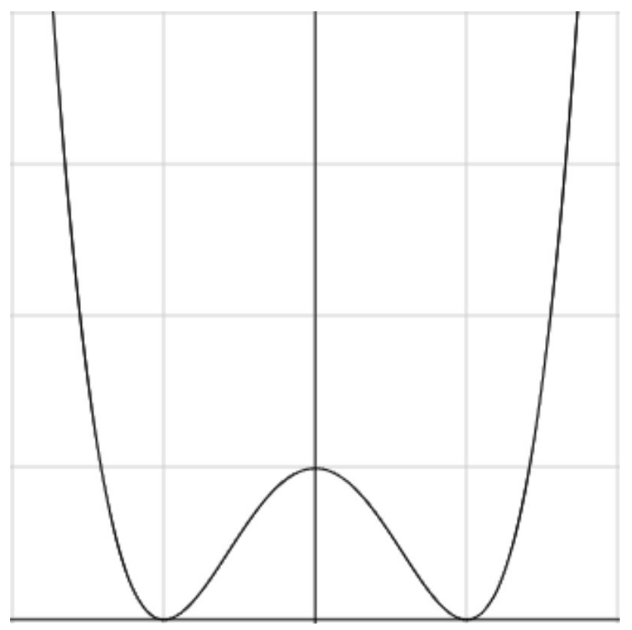
\includegraphics[scale=0.5]{higgsPotential.png}
   \caption{Higgs Potential where the y-axis has units of energy and the x-axis is the scalar field.}
   \label{fig:fig_1-8}
\end{figure}
In order to finish off our rules for creating Feynman diagrams we can draw the interaction vertex for the Higgs Boson in Figure \ref{fig:fig_1-9}. 
It can interact with any massive particle, including itself. 
The Higgs Boson has no charge, no spin and a mass of 126 $\frac{GeV}{c^2}$.

\begin{figure} %  figure placement: here, top, bottom, or page
   \centering
      \feynmandiagram[horizontal=a to b] {
         i1  [particle=particle with mass] -- [fermion] a -- [fermion] i2  [particle=particle with mass],
         a -- [scalar, edge label=Higgs] b, 
      };
   \caption{Higgs Boson Vertex.}
   \label{fig:fig_1-9}
\end{figure}
\clearpage
\section{Gauge Field}

A gauge field is the mathematical mechanism behind the SM forces. A gauge theory is a type of field theory for which the Lagrangian\footnote{The lagrangian is a mathematical formalism for writing out all the interactions in a field theory through the action (the spatial integration of the lagrangian density) of the fields. The SM lagrangian is shown in Figure \ref{fig:fig_1-1}.} does not change for local transformations. 
QCD, and QED are gauge field theories. The local symmetry that the SM is invariant under is $U(1)\times SU(2)\times SU(3)$ where U stands for unitary and S stands for special.
Although the mathematics of this local symmetry are beyond the scope of this thesis, the consequences are important to note.

For example, the mathematical reason that there are eight gluons in QCD is because SU(3), the symmetry of QCD, has eight generators. QED is the U(1) symmetry and the weak force is under the SU(2) symmetry.
Therefore, the $U(1)\times SU(2)\times SU(3)$ symmetry encompasses all three fundamental forces of the SM. 
The combined symmetry generates 12 gauge bosons, the bosons which corresponds to the gauge field, which we now know as the photon, the 3 bosons of the weak force, and the 8 gluons.

\section{What's Left?}

Now that we have a good understanding of the SM, we can make a vast number of theoretical predictions.  All such predictions have, so far, been confirmed by experiments. 
Unfortunately, it isn't complete. 
Gravity is noticeably absent. Our current understanding of gravity, through the theory of General Relativity, does not mesh nicely with the equations of the SM. Large and complicated theoretical efforts have been working very hard to try to reconcile this difference but it still remains today. 

Beyond that, the visible matter in our universe only makes up about 4\% of the stuff in it. Physicists have good evidence that the universe is roughly 25\% matter so what is the other 21\%?
This extra stuff is theorized to be ``dark matter'', i.e. not interacting in a way we can directly detect, and is not currently included in the SM. There are many theories and experiments working on this question.
After that, we still don't understand the other approximately 75\% of the rest of the universe. Is it the so called ``dark energy''? We know even less about this than we do about dark matter.

Another problem is that we don't even fully understand the roughly 4\% of baryonic matter we do know about. The majority of this matter is made of particles but why? Why are there not more anti particles? It is not clear why there would be an asymmetry to the amount of matter vs anti matter. 
Some progress has been made recently on this question but the answer is still incomplete. It was previously stated that we don't have a good measurable of the neutrino masses. This is also a open question because it is not clear whether or not they are massless.

There are also there are theoretical inconsistencies in the SM. One example is that the quantum corrections to the Higgs mass are 18 order of magnitude larger than the measured value of the Higgs mass. 
This is called the Hierarchy problem and will be detailed more in the next chapter. There is also an unmeasured Higgs quantity, the shape of the curvature of the Higgs potential.
This is the last unmeasured parameter in the SM.

So given that we seem to be missing many answers to questions about known measurable physical phenomenon, how do we explain them? Theorists spend their days creating answers for these questions in a manner that would be consistent with the current SM.
These theories are know as ``Beyond Standard Model'' (BSM) and can address one or all of the known issues with the SM. Now we shall talk about a few BSM theories that will be relevant to this experiment.